% This is "sig-alternate.tex" V2.1 April 2013
% This file should be compiled with V2.5 of "sig-alternate.cls" May 2012
%
% This example file demonstrates the use of the 'sig-alternate.cls'
% V2.5 LaTeX2e document class file. It is for those submitting
% articles to ACM Conference Proceedings WHO DO NOT WISH TO
% STRICTLY ADHERE TO THE SIGS (PUBS-BOARD-ENDORSED) STYLE.
% The 'sig-alternate.cls' file will produce a similar-looking,
% albeit, 'tighter' paper resulting in, invariably, fewer pages.
%
% ----------------------------------------------------------------------------------------------------------------
% This .tex file (and associated .cls V2.5) produces:
%       1) The Permission Statement
%       2) The Conference (location) Info information
%       3) The Copyright Line with ACM data
%       4) NO page numbers
%
% as against the acm_proc_article-sp.cls file which
% DOES NOT produce 1) thru' 3) above.
%
% Using 'sig-alternate.cls' you have control, however, from within
% the source .tex file, over both the CopyrightYear
% (defaulted to 200X) and the ACM Copyright Data
% (defaulted to X-XXXXX-XX-X/XX/XX).
% e.g.
% \CopyrightYear{2007} will cause 2007 to appear in the copyright line.
% \crdata{0-12345-67-8/90/12} will cause 0-12345-67-8/90/12 to appear in the copyright line.
%
% ---------------------------------------------------------------------------------------------------------------
% This .tex source is an example which *does* use
% the .bib file (from which the .bbl file % is produced).
% REMEMBER HOWEVER: After having produced the .bbl file,
% and prior to final submission, you *NEED* to 'insert'
% your .bbl file into your source .tex file so as to provide
% ONE 'self-contained' source file.
%
% ================= IF YOU HAVE QUESTIONS =======================
% Questions regarding the SIGS styles, SIGS policies and
% procedures, Conferences etc. should be sent to
% Adrienne Griscti (griscti@acm.org)
%
% Technical questions _only_ to
% Gerald Murray (murray@hq.acm.org)
% ===============================================================
%
% For tracking purposes - this is V2.0 - May 2012

\documentclass{sig-alternate-05-2015}
\usepackage{times}
\usepackage{helvet}
\usepackage{courier}
\usepackage{graphicx}
\usepackage{booktabs} % for pretty table rules
\usepackage{hyperref}
\usepackage[T1]{fontenc}

\setlength{\pdfpagewidth}{8.5in}
\setlength{\pdfpageheight}{11in}
\pdfinfo{
/Title Monitoring the Gender Gap with Wikidata Human Gender Indicators
/Author BLINDED}

\begin{document}

% Copyright
\setcopyright{acmcopyright}
%\setcopyright{acmlicensed}
%\setcopyright{rightsretained}
%\setcopyright{usgov}
%\setcopyright{usgovmixed}
%\setcopyright{cagov}
%\setcopyright{cagovmixed}


% DOI
\doi{10.475/123_4}

% ISBN
\isbn{123-4567-24-567/08/06}

%Conference
\conferenceinfo{PLDI '13}{June 16--19, 2013, Seattle, WA, USA}

\acmPrice{\$15.00}

%
% --- Author Metadata here ---
\conferenceinfo{WOODSTOCK}{'97 El Paso, Texas USA}
%\CopyrightYear{2007} % Allows default copyright year (20XX) to be over-ridden - IF NEED BE.
%\crdata{0-12345-67-8/90/01}  % Allows default copyright data (0-89791-88-6/97/05) to be over-ridden - IF NEED BE.
% --- End of Author Metadata ---

\title{Monitoring the Gender Gap with Wikidata Human Gender Indicators}

%
% You need the command \numberofauthors to handle the 'placement
% and alignment' of the authors beneath the title.
%
% For aesthetic reasons, we recommend 'three authors at a time'
% i.e. three 'name/affiliation blocks' be placed beneath the title.
%
% NOTE: You are NOT restricted in how many 'rows' of
% "name/affiliations" may appear. We just ask that you restrict
% the number of 'columns' to three.
%
% Because of the available 'opening page real-estate'
% we ask you to refrain from putting more than six authors
% (two rows with three columns) beneath the article title.
% More than six makes the first-page appear very cluttered indeed.
%
% Use the \alignauthor commands to handle the names
% and affiliations for an 'aesthetic maximum' of six authors.
% Add names, affiliations, addresses for
% the seventh etc. author(s) as the argument for the
% \additionalauthors command.
% These 'additional authors' will be output/set for you
% without further effort on your part as the last section in
% the body of your article BEFORE References or any Appendices.

\numberofauthors{5} %  in this sample file, there are a *total*
% of EIGHT authors. SIX appear on the 'first-page' (for formatting
% reasons) and the remaining two appear in the \additionalauthors section.
%
\author{
% You can go ahead and credit any number of authors here,
% e.g. one 'row of three' or two rows (consisting of one row of three
% and a second row of one, two or three).
%
% The command \alignauthor (no curly braces needed) should
% precede each author name, affiliation/snail-mail address and
% e-mail address. Additionally, tag each line of
% affiliation/address with \affaddr, and tag the
% e-mail address with \email.
%
% 1st. author
\alignauthor
Author Blinded\\
       \affaddr{blind}\\
       \affaddr{blind}\\
       \affaddr{blind}\\
       \email{blind}
% 2nd. author
\alignauthor
Author Blinded\\
       \affaddr{blind}\\
       \affaddr{blind}\\
       \affaddr{blind}\\
       \email{blind}
% 3rd. author
\alignauthor 
Author Blinded\\
       \affaddr{blind}\\
       \affaddr{blind}\\
       \affaddr{blind}\\
       \email{blind}
\and  % use '\and' if you need 'another row' of author names
% 4th. author
\alignauthor 
Author Blinded\\
       \affaddr{blind}\\
       \affaddr{blind}\\
       \affaddr{blind}\\
       \email{blind}
% 5th. author
\alignauthor 
Author Blinded\\
       \affaddr{blind}\\
       \affaddr{blind}\\
       \affaddr{blind}\\
       \email{blind}
}
% There's nothing stopping you putting the seventh, eighth, etc.
% author on the opening page (as the 'third row') but we ask,
% for aesthetic reasons that you place these 'additional authors'
% in the \additional authors block, viz.
% Just remember to make sure that the TOTAL number of authors
% is the number that will appear on the first page PLUS the
% number that will appear in the \additionalauthors section.

\maketitle
\begin{abstract}
The gender gap in Wikipedia's content, specifically in the reperesentation of women in biographies is well-known, but has been difficult to measure and monitor its evolution. There exist efforts to address this gender gap, but the impacts they are having have received no attention. To investigate we utilise Wikidata, the database that feeds Wikipedia, and introduce the ``Wikidata Human Gender Indicators'' (WHGI), an open source, open data, real time, longitudinal, biographical dataset that can provide insights into gender disparities across time, space, culture, occupation and language. Through these lenses we show how women's representation has changed along 11 dimensions. Furthermore, to demonstrate it's more general use in research we present validations of the WHGI against three exogenous datasets: the world's historical population, ``traditional'' gender-disparity indices (GDI, GEI, GGGI and SIGI), and occupational gender according to the US Bureau of Labor Statistics.
\end{abstract}


%
% The code below should be generated by the tool at
% http://dl.acm.org/ccs.cfm
% Please copy and paste the code instead of the example below. 
%
\begin{CCSXML}
<ccs2012>
 <concept>
  <concept_id>10010520.10010553.10010562</concept_id>
  <concept_desc>Example</concept_desc>
  <concept_significance>500</concept_significance>
 </concept>

\end{CCSXML}

\ccsdesc[500]{Computer systems organization~Example}
\ccsdesc[300]{Computer systems organization~Redundancy}
\ccsdesc{Computer systems organization~Robotics}
\ccsdesc[100]{Networks~Network reliability}


%
% End generated code
%

%
%  Use this command to print the description
%
\printccsdesc

% We no longer use \terms command
%\terms{Theory}

\keywords{ACM proceedings; \LaTeX; text tagging}

\section{Introduction}

Gender inequality is a long-standing social problem which affects many aspects of society. Worldwide, cultural ideologies have created scenarios which make women more prone to health issues \cite{world_health_organization_women_2009}. Likewise in education attitudes create a systemic gender bias in opportunity \cite{heward_gender_1999}. And, famously, incomes for identical jobs are lower for women \cite{burstein_equal_????}.

Statistical gender indicators are critically important to understanding gender inequality, but their construction is difficult \cite{klasen_gender-related_2004}. Many indicators (single measures) and indices (compound measures) have been proposed, such as The Gender Development Index from the United Nations Development and the Global Gender Gap Index from the World Economic Forum, but no academic consensus exists on which is superior \cite{hawken_cross-national_2012}. Owing to this varied landscape using a plurality of inhat dicators is recommended for research \cite{jutting_measuring_2008}.

We introduce an open source, open data, real-time, intersectional dataset that can provide insights into gender disparities across time, space, culture, occupation and language. ``Wikidata Human Gender Indicators'' (WHGI) is a  dataset consiting  of 11 separate indicators on the gender representation of humans in Wikidata.

Measuring and releasing data on Wikipedia's content gender gap attempts to solve two problems. The scope of Wikipedia, and the advent of its machine-readability through Wikidata, gives us an unprecedented look at gender at a scale never seen before. This provides potential for applications not possible until now. Secondly, we wish to shed light on Wikipedia's data under the philosophy of ``what gets measured, gets fixed.''

The thread of research on Wikipedia's gender biases originates in the finding that Wikipedia's editors are largely not women \cite{hill_wikipedia_2013}. This imbalance has been attributed to an internet skills gap \cite{hargittai_mind_2015} and its internal culture \cite{lam_wp:clubhouse?:_2011}. 

More and more, in addition to investigations of the Wikipedia \textit{editor gender gap} researchers have also been interrogating the character of its \textit{biography gender gap}. Early studies found that Wikipedia excluded notable women more than its counterparts \cite{reagle_gender_2011}. More recently \cite{wagner_its_2015} showed that while coverage of women in large Wikipedias is not less than other reference works, the language with which women are portrayed is different and focuses more on romance and family. Women also tend to be less central in the link graph of Wikipedia \cite{10.1371/journal.pone.0114825}. These linguistic and network findings were confirmed by \cite{graells-garrido_first_2015}, who also showed evidence of stereotyping in metadata.

Yet in popular mindshare there persists a sentiment that denies that any of this is a problem \cite{eckert_retriggering_2013}. Luckily, experiments are showing that awareness of Wikipedia's gender issues is a strategy that can alleviate the problem \cite{hinnosaar_gender_2015}, for which more methods are always needed.

Wikidata, the database that feeds Wikipedia, offers new opportunities to analyze culture programmatically. Launched in 2012, Wikidata is designed to host structured data that is \textit{multilingual} (so there is only one edition) and \textit{plural} (can support many competing facts) \cite{vrandecic_wikidata:_2014}.  These features make Wikidata the perfect place for all Wikipedias to collaboratively store facts about the world. If an Italian Wikipedian stores information about the population of ancient Rome, that information is then available to every other Wikipedia with a short code snippet. Every language collaborating together has meant that Wikidata has become a massive free open knowledgebase in its own right, containing over 40 million facts \cite{krotzsch_how_????}.

As a knowledgebase, Wikidata is slowly proving its worth for research. For instance, Wikidata has been used to find popular connections between nationalities and occupations \cite{goldfarb_quantifying_2015}. Or take the fact that all human and mouse genes have been imported into Wikidata \cite{mitraka_wikidata:_2015}, for an internet-wide community effort to find links between genes, drugs and diseases \cite{burgstaller-muehlbacher_wikidata_2015}. All of these tasks would be difficult to do without Wikidata.

\subsection{Outline}

This paper begins by describing the format of Wikidata and statistics of humans contained in it. We investigate how gender composition and data quality has changed over time and demonstrate the impact that WHGI can have as a metric for content and women-focused Wikipedian communities.  

Moving beyond Wikipedia navel-gazing, we present 3 validation measures utilizing ground truths from the US Census Bureau, Bureau for Labor Statistics, and United Nations Development Program. We show that WHGI does in fact relate to the real world. This means that, albeit imperfectly, the WHGI can be a proxy for numerical data about the real word in times and places for which no previous data exists.


\section{Humans in Wikidata}

Wikidata is a general database consisting of \textit{items} which are described by \textit{properties} that take on \textit{values}. Our interest is in biographies of people, that is any item which has the property \textit{instance of} with value \textit{human} \footnote{As Wikidata is intentionally multilingual, itesm, properties and values are actually reference by number. So ``instance of: human'' is ``P31:Q5'' in Wikidata terms }). For each human item we find the corresponding values of \textit{gender}, \textit{date of birth}, \textit{date of death}, \textit{place of birth}, \textit{citizenship}, \textit{ethnic group}, \textit{field of work}, and \textit{occupation} \footnote{These correspond to Wikidata properties P21, P569, P570, P19, P27, P172, P101, and P106 respectively.} In Figure \ref{fig:aung}, we illustrate the semantics of a Wikidata Human on the item for Aung San Suu Kyi.

\begin{figure}
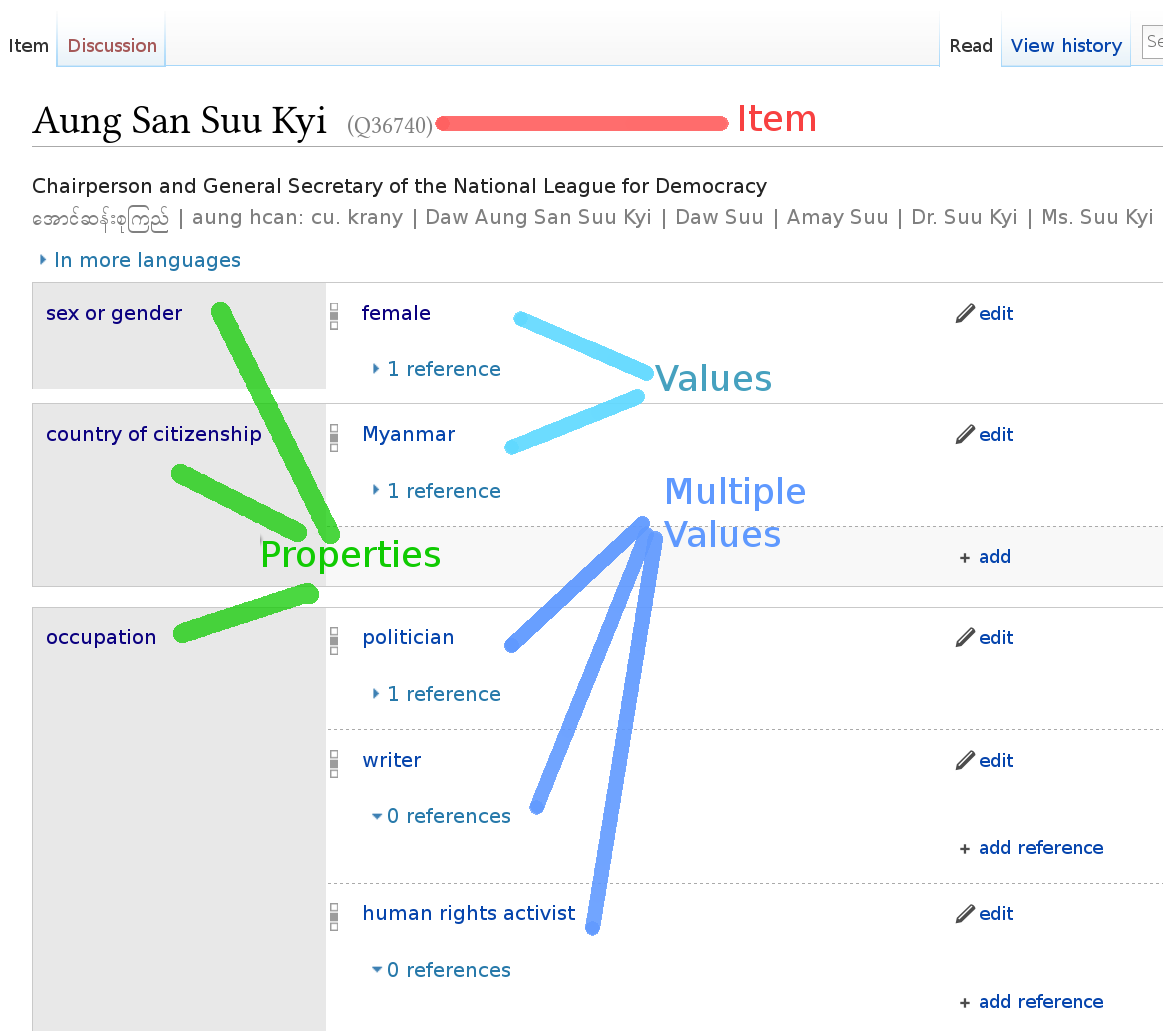
\includegraphics[scale=0.2]{figures/aung_explainer_small.png} 
\caption{Example Wikidata Human Item of Aung San Suu Kyi}
\label{fig:aung}
\end{figure}
 
\begin{table}
\caption{A small excerpt of the January 3\textsuperscript{rd} 2016 date of birth indicator illustrating the gender aggregation of Wikidata by birth year. The earliest humans in Wikidata are two men born in 4203 b.c.e., there are many notable births in the 1980's (see Figure \ref{fig:genderbydob}), and there are thirteen notable 1-year-olds in Wikidata. Notice the inclusion of non-binary genders as they are recorded in Wikidata, as well as biographies without any gender recorded.}
\begin{tabular} {p{0.8cm}p{0.8cm}p{0.8cm}p{0.8cm}p{0.8cm}p{0.8cm}p{0.8cm}}
\toprule
date of birth & no gender & trans-gender female & gender-queer & ka-thoey & female & male \\
\midrule
4203 \small{(B.C.E.)} & & & & & & 2   \\ 
$\cdots$ &  &  &  & &  &    \\ 
1981 & 849 & 1 &  & 1 &5,042 & 14,461 \\ 
1982 & 861 & 2 &  & &5,132 & 14,372  \\ 
1983 & 864 & 3 &  & &5,078 & 14,520  \\ 
1984 & 830 & 3 & 1 & &5,372 & 14,558   \\ 
1985 & 777 & 4 &  & &5,400 & 14,664  \\ 
$\cdots$ &  &  &  & &  &    \\ 
2015 & 6 &  &  & & 4 & 3  \\ 
\bottomrule
\end{tabular}
\label{table:dob}
\end{table}
For each of the above eight properties we create an ``indicator'' by aggregating the dataset on that property, but disaggregate by gender. Take for example the date of birth indicator, it has one row per year found as a date of birth, and one column per gender represented in Wikidata. See a sample excerpt of the date of birth indicator in Table \ref{table:dob}, and it's visualization in \ref{fig:genderbydob}. In addition to the eight indicators made directly from properties, we include three more which feature augmented data. There is a indicator based on the Wikipedia languages in which a human is represented. And we include a geographic aggregation of citizenship, place of birth and ethnic group into indicators called \textit{culture}, and \textit{worldmap}. See Figure \ref{fig:genderbycountry} for the worldmap visualization. 


\begin{figure}
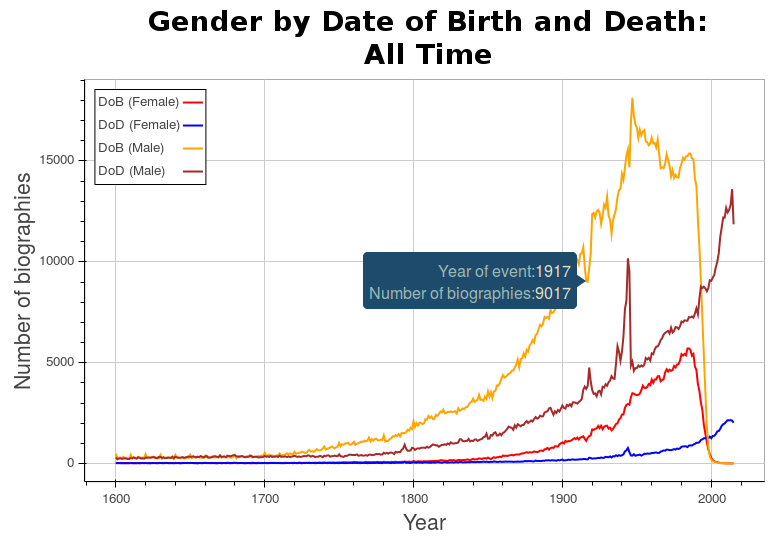
\includegraphics[scale=0.31]{figures/genderbydob.png} 
\caption{The total of Wikidata gendered biographies aggregated by date of birth and date of death. This data is represents the January 3\textsuperscript{rd} 2016 snapshot. See the noticable spikes in death for men around World War II, and that births of both genders drop about 20 years before the current year, as younger people tend not to be notable.}
\label{fig:genderbydob}
\end{figure}

\begin{figure}
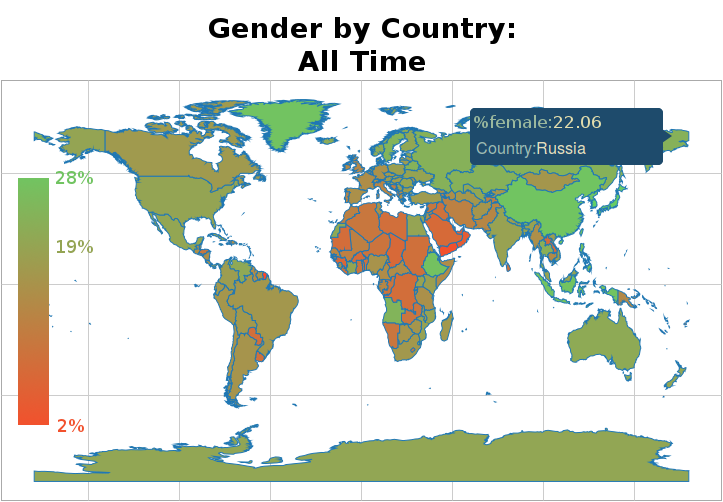
\includegraphics[scale=0.33]{figures/genderbycountry.png} 
\caption{The Wikidata female ratio of biographies aggregated by place of birth and citizenship. This data is represents the January 3\textsuperscript{rd} 2016 snapshot.}
\label{fig:genderbycountry}
\end{figure}

\begin{figure}
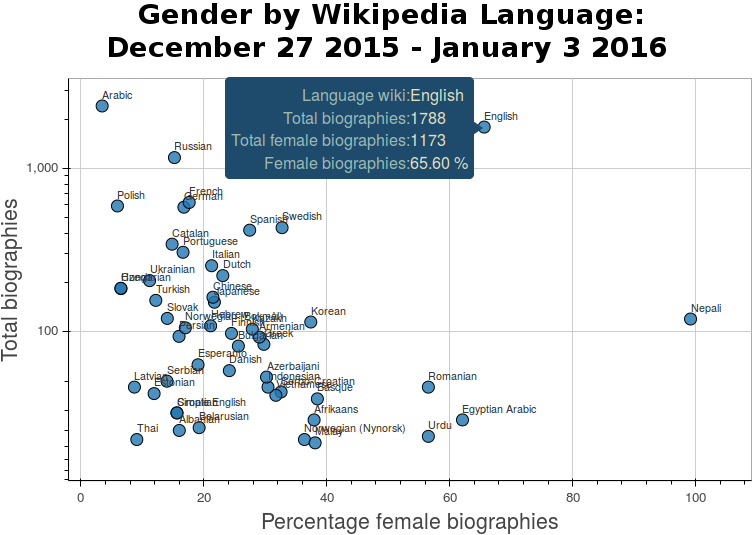
\includegraphics[scale=0.31]{figures/genderbylang.png} 
\caption{The changes in the size and percentage of female biographies for large Wikipedia languages in the period December 27\textsuperscript{th} 2015 - January 3\textsuperscript{rd} 2016. English Wikipedia Increased 1,788 biographies 65\% of which were about women. Meanwhile Nepali Wikipedia increased by 120 biographies, 119 of which were about women.}
\label{fig:genderbylang}
\end{figure}

\subsection{Snapshots}
All of our data is dervied from the official Wikidata database downloads, which represent a cross-sectional ``snapshot'' of Wikidata as it was at a specific date. Wikidata releases a new snapshot weekly. We re-process each of the 11 indicators for every new snapshot, and additionally compute the differences that occured between the newest snapshot and the second-newest. This allows us to monitor activity on Wikidata at a weekly level of granularity. For instance Figure  \ref{fig:genderbydob} and Figure \ref{fig:genderbycountry} show the state of the date of birth and country indicators, \textit{for all time}, as of the January 3\textsuperscript{rd} 2016 snapshot. However Figure \ref{fig:genderbylang} shows the \textit{changes} of the week between December 27\textsuperscript{th} 2015 - January 3\textsuperscript{rd} 2016.

Therefore we are also generating a dataset of \textit{weekly changes} which allows us to monitor the status of biographies in Wikidata. We can inspect the changes in composition of genders, or date of birth, which can speak to efforts from Wikipedian communities attempting to counter bias in the database. 

\subsection{Technical Details}

Note that for fidelity there is virtually no data-cleaning done, as the point of our project is to display information as faithfully as possible. Our dataset is meant to be used to uncover potential biases in Wikidata and the world at large, and we feel that any cleaning process would introduce further biases. An instructive illustration of this case is that the ``gender'' property in Wikidata is actually labelled in English  as ``sex or gender'' (no distinction), and not limited to any value. Over our time snapshotting we found 36 values used for ``sex or gender'', including ``male'' and ``female'', but extending to nonbinary genders ``transgender female'', ``intersex'', ``fa'afafine'', ``transgender'', ``Gender fluid'',  ``genderqueer'', ``kathoey'', and ``queer''. At times the other categories of information are recorded here - perhaps erroneously - such as ``gay'', or ``homosexuality''. And even what seem to be mistakes are left in, such as one-offs of ``Solanum tuberosum'', ``Messi'', or ``sociologist''. Cleaning this data would be a disservice, we feel, to communicating how - and how well - Wikidata is used.


Our dataset and code used to generate it is available for free under the CC-BY license online. Our first snapshot is from September 17\textsuperscript{th} 2014, and tracks the official  Wikidata data dumps, updating weekly. We archived the January 3\textsuperscript{rd} 2016 version as a quality-checked, canonical version \footnote{\url{WEBSITE BLINDED}}. All our code to make this data and the analyses presented here SVs and generate the following results using both \textit{python-pandas} and \textit{R} can be found in our github repository \footnote{\url{WEBSITE BLINDED}}.

Note that the missing data in the first half of 2015 is due to  the period in which we were building the automation of collecting these statistics. 


\section{Longitudinal Statistics}
A main purpose for investigating this dataset is to support and provide metrics for Wikipedians communities attempting to  address content gaps. Therefore we turn to focus at statistics of our dataset with regard to how it has changed over time as these Wikipedian communities have been edting. 

\begin{figure}
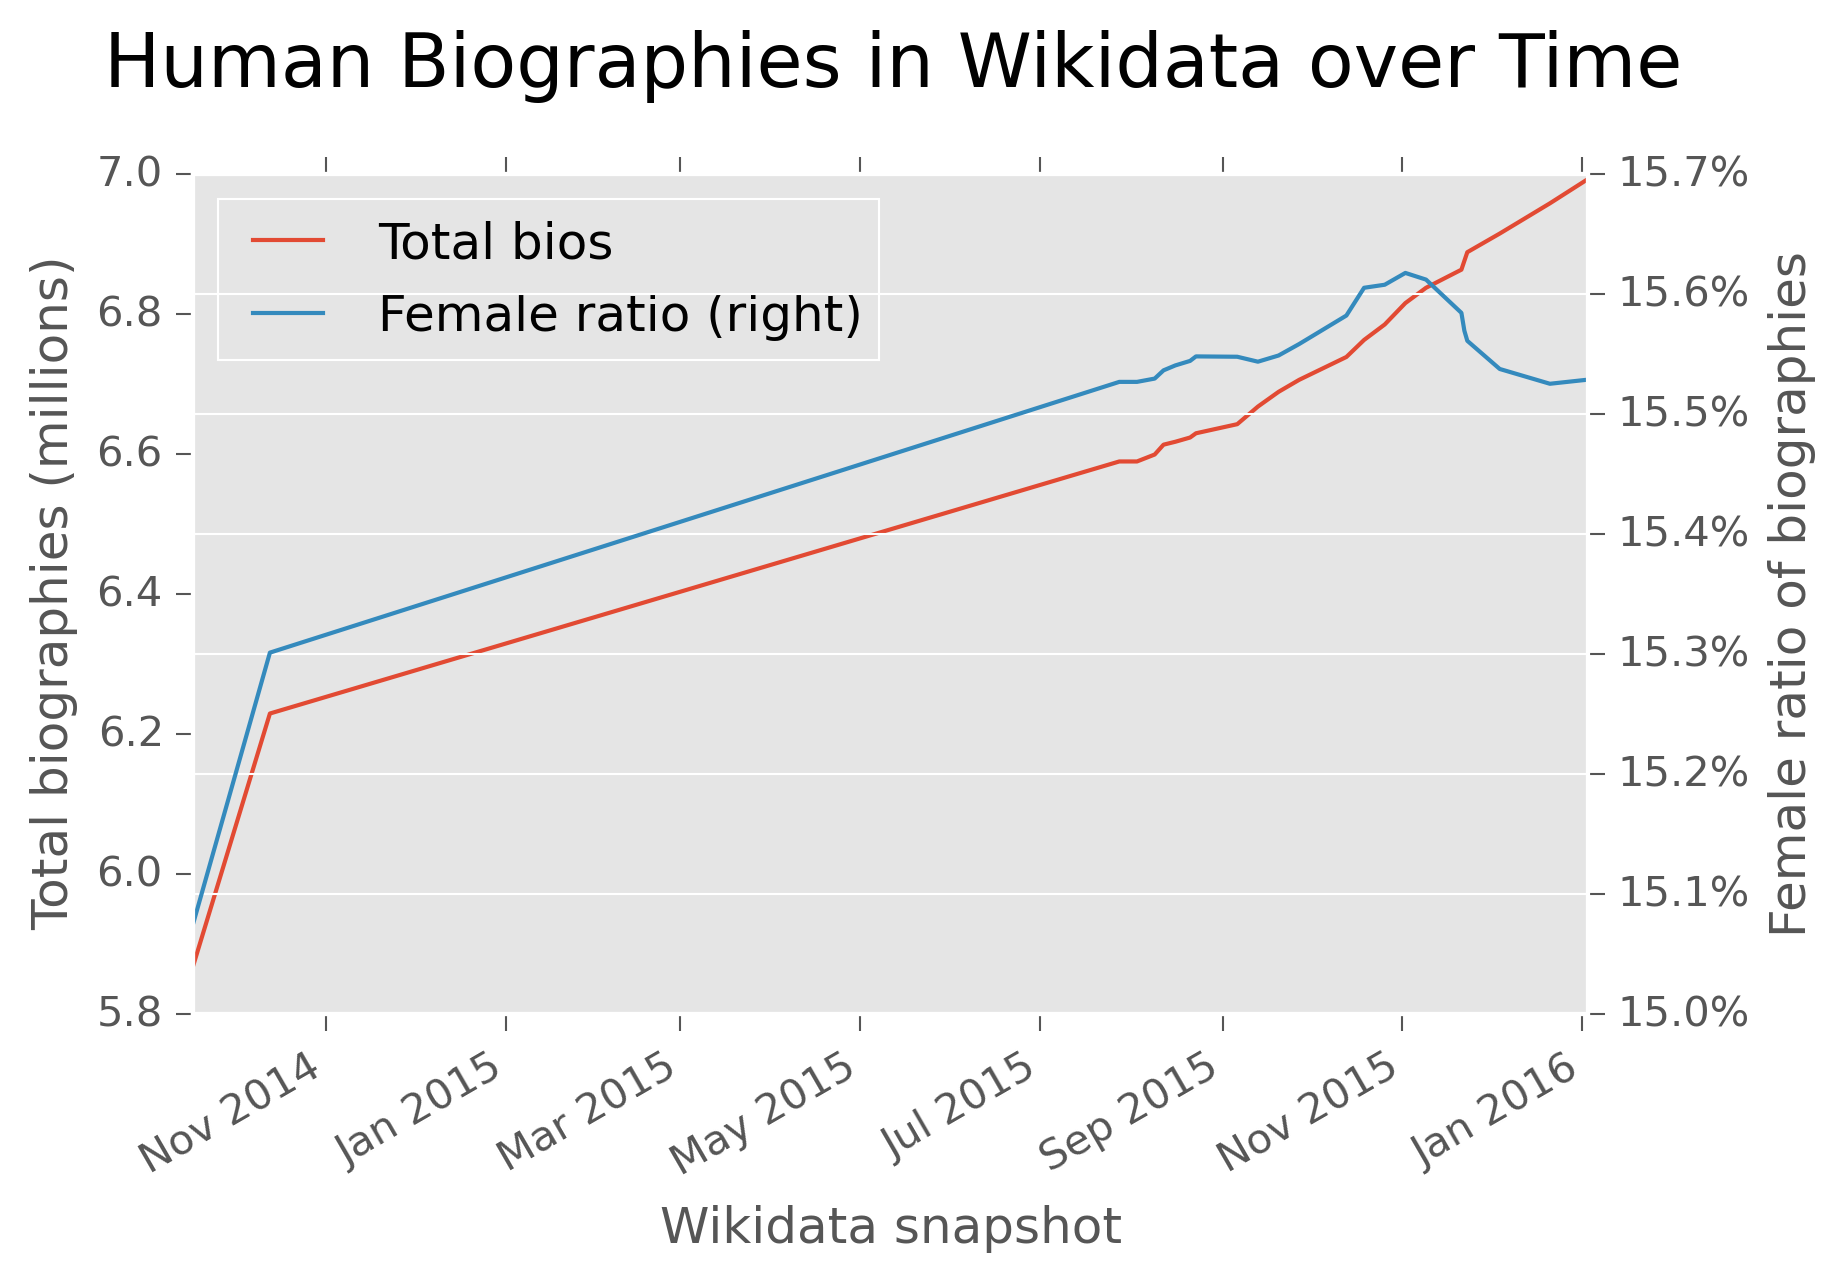
\includegraphics[scale=0.53]{figures/totalfrb.png} 
\caption{Total number of human biographies (left) and the female ratio of those biographies (right) by Wikidata snapshot. The total number of humans found in Wikidata over time is displaying linear, unconstrained growth. Over the same  the female ratio of biographies in Wikidata has risen by 0.5\%.}
\label{fig:totalfrb}
\end{figure}

First we queried the way the total number of biographies and the ratio of women represented as Wikidata has evolved. Total humans in Wikidata increased from 5,869,606 to 6,999,542, and shows linear, unconstrained growth (see Figure \ref{fig:totalfrb}). Certainly Wikidata is activte and changing, but how? An important measure for content-focused communities is the ratio of biographies which are about women, as espoused in \textit{WikiProject Women in Red}\footnote{\url{https://en.wikipedia.org/wiki/Wikipedia:WikiProject_Women_in_Red}}. We looked into the ratio of  humans recorded ``female'' versus all gendered biographies. Similar to total biographies this measure is rising at a fairly linear rate of approximately 0.5\% per year\ref{fig:totalfrb}. The final months on record show a slight decline which warrants further investigation. 


\begin{figure}
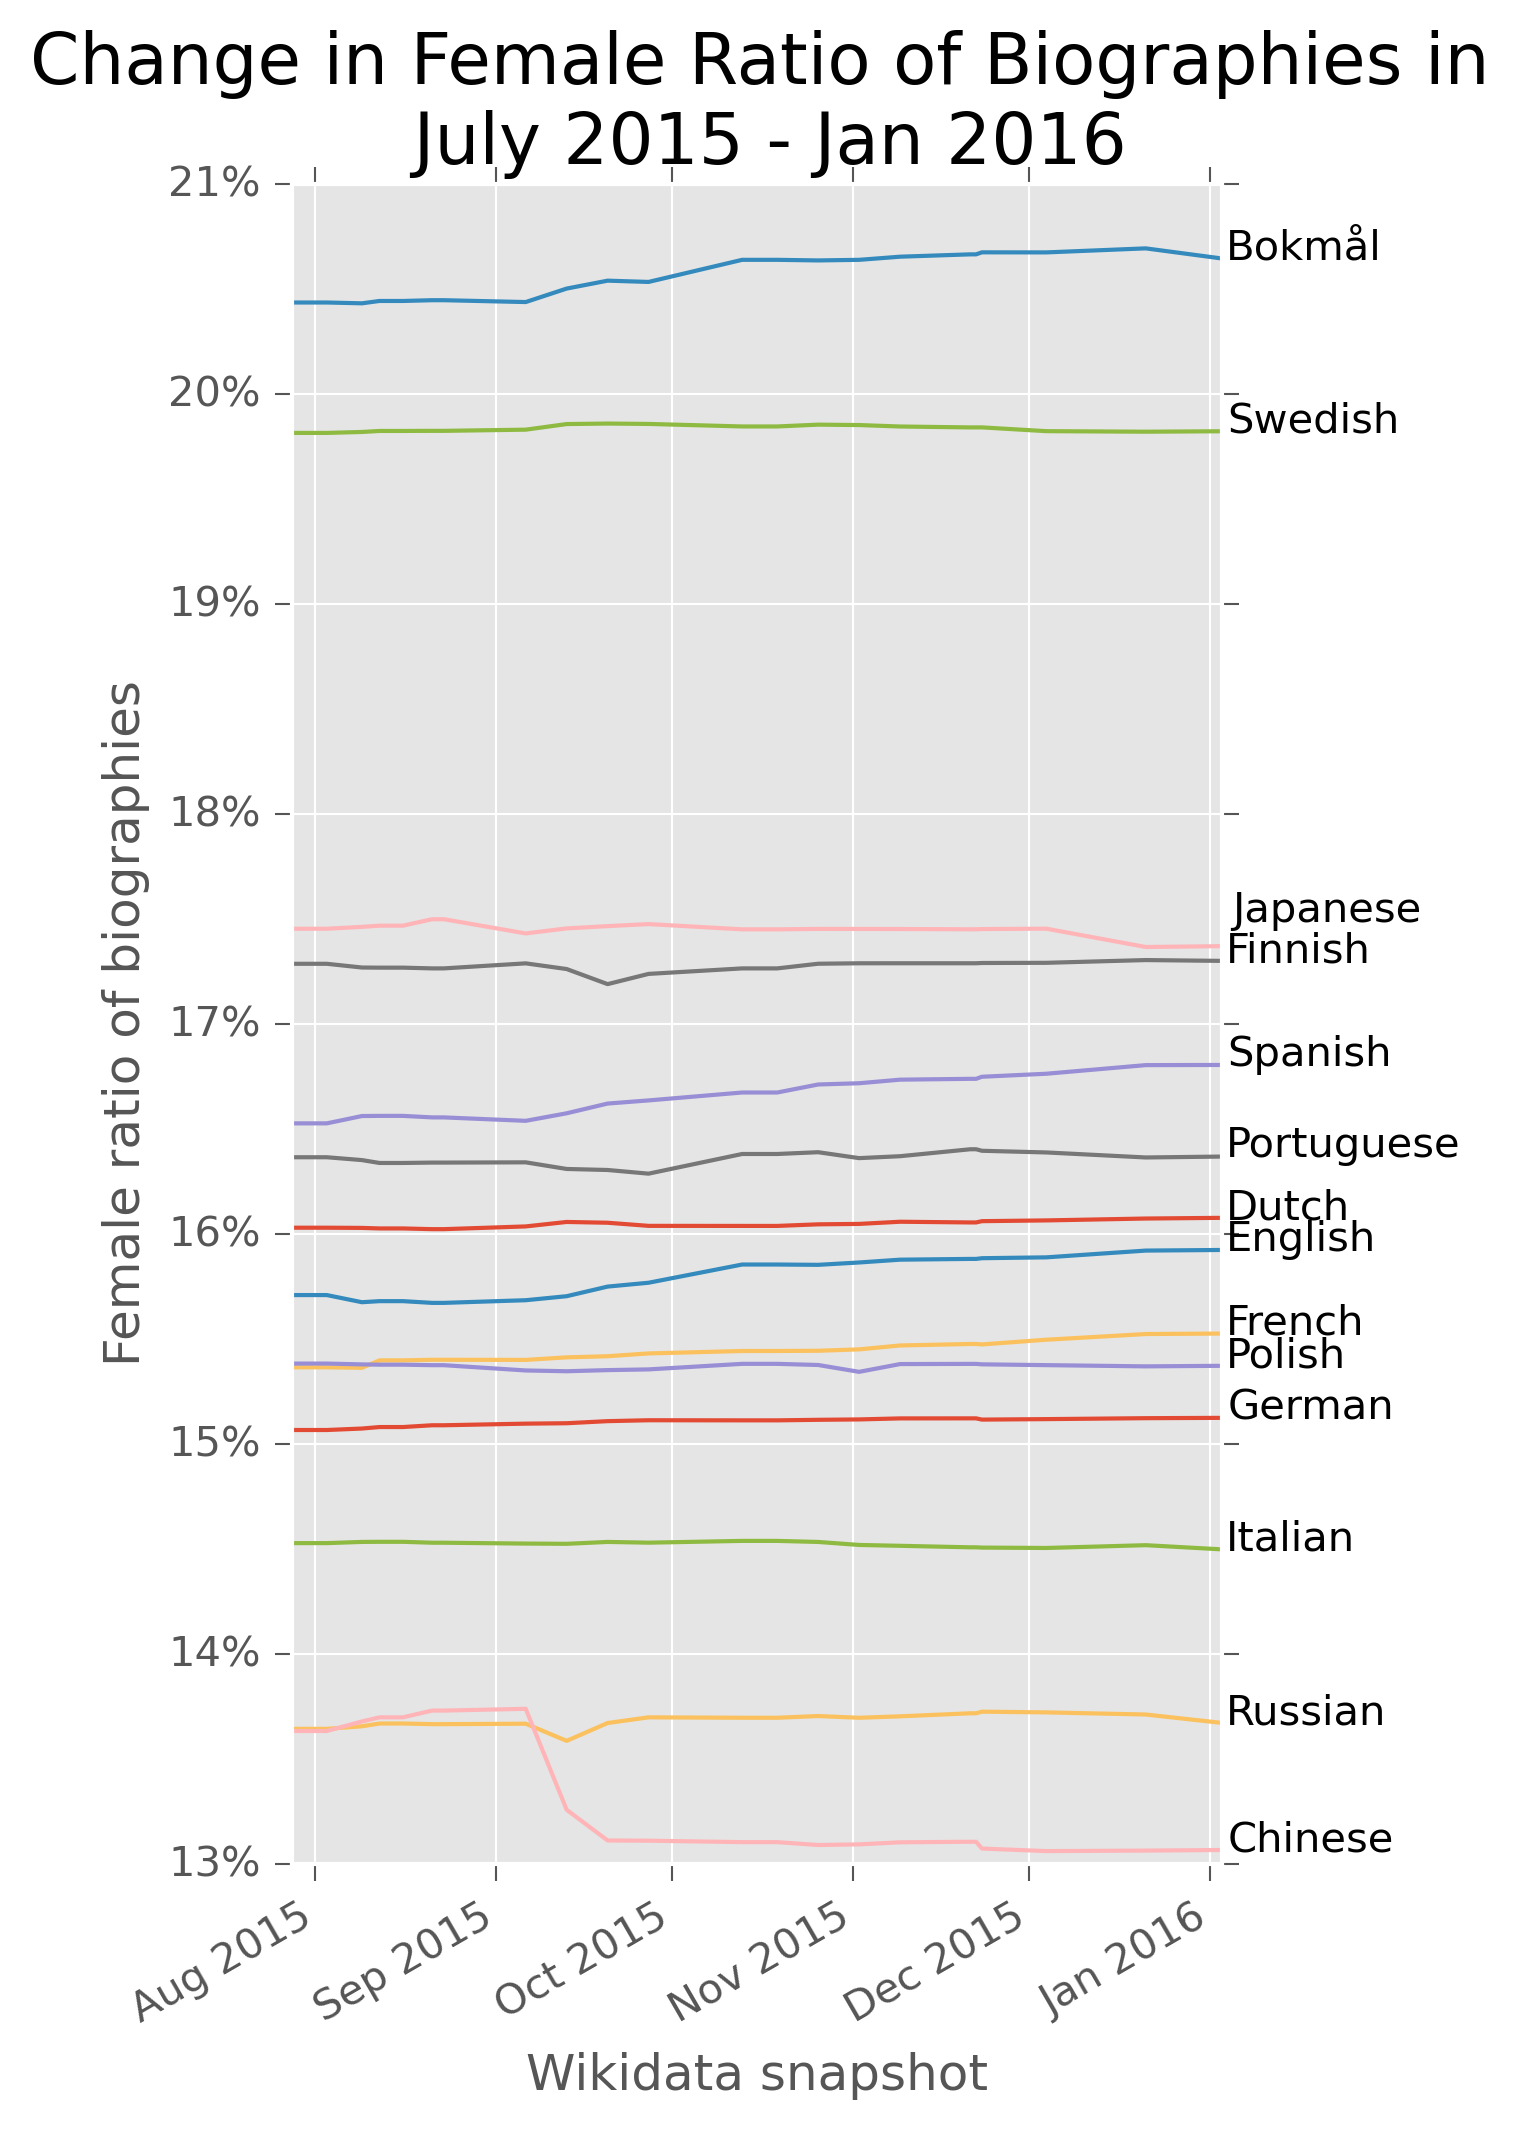
\includegraphics[scale=0.6]{figures/changefrb.png} 
\caption{The change in female ratio of biographies over time, by Wikipedia languages with 100,000 or more gendered biographies. Even during this short time period, the Norwegian (Bokm\aa l), Spanish, and English Wikipedias all show visible up-ticks in representing Women.}
\label{fig:changefrb}
\end{figure}

We took a more granular look at the evolution of the female ratio of biographies by disaggregating by Wikipedia Language in Figure \ref{fig:changefrb}. Of the languages that have 100,000 or more gendered biographies, and during the time period July 2015, to January 2016, we see the rate of women in Norwegian (Bokm\aa l), Spanish, and English Wikipedias each increase by more than 0.25\%.

Fortunately Wikiproject Women in Red keeps metrics of how many biographies they added on a monthly basis, and we were able to conduct a cross-correlation between the monthly number of biographies created by Women in Red, and the number of female biographies added to English Wikipedia. The correlation between these activities is 0.657, which indicates that they are indeed related. Unfortunately we cannot determine a casual relationship between editing efforts and the increase in women's representation in these languages. Still we are able to numerically highlight this trend which was not viewable before.


\begin{figure}
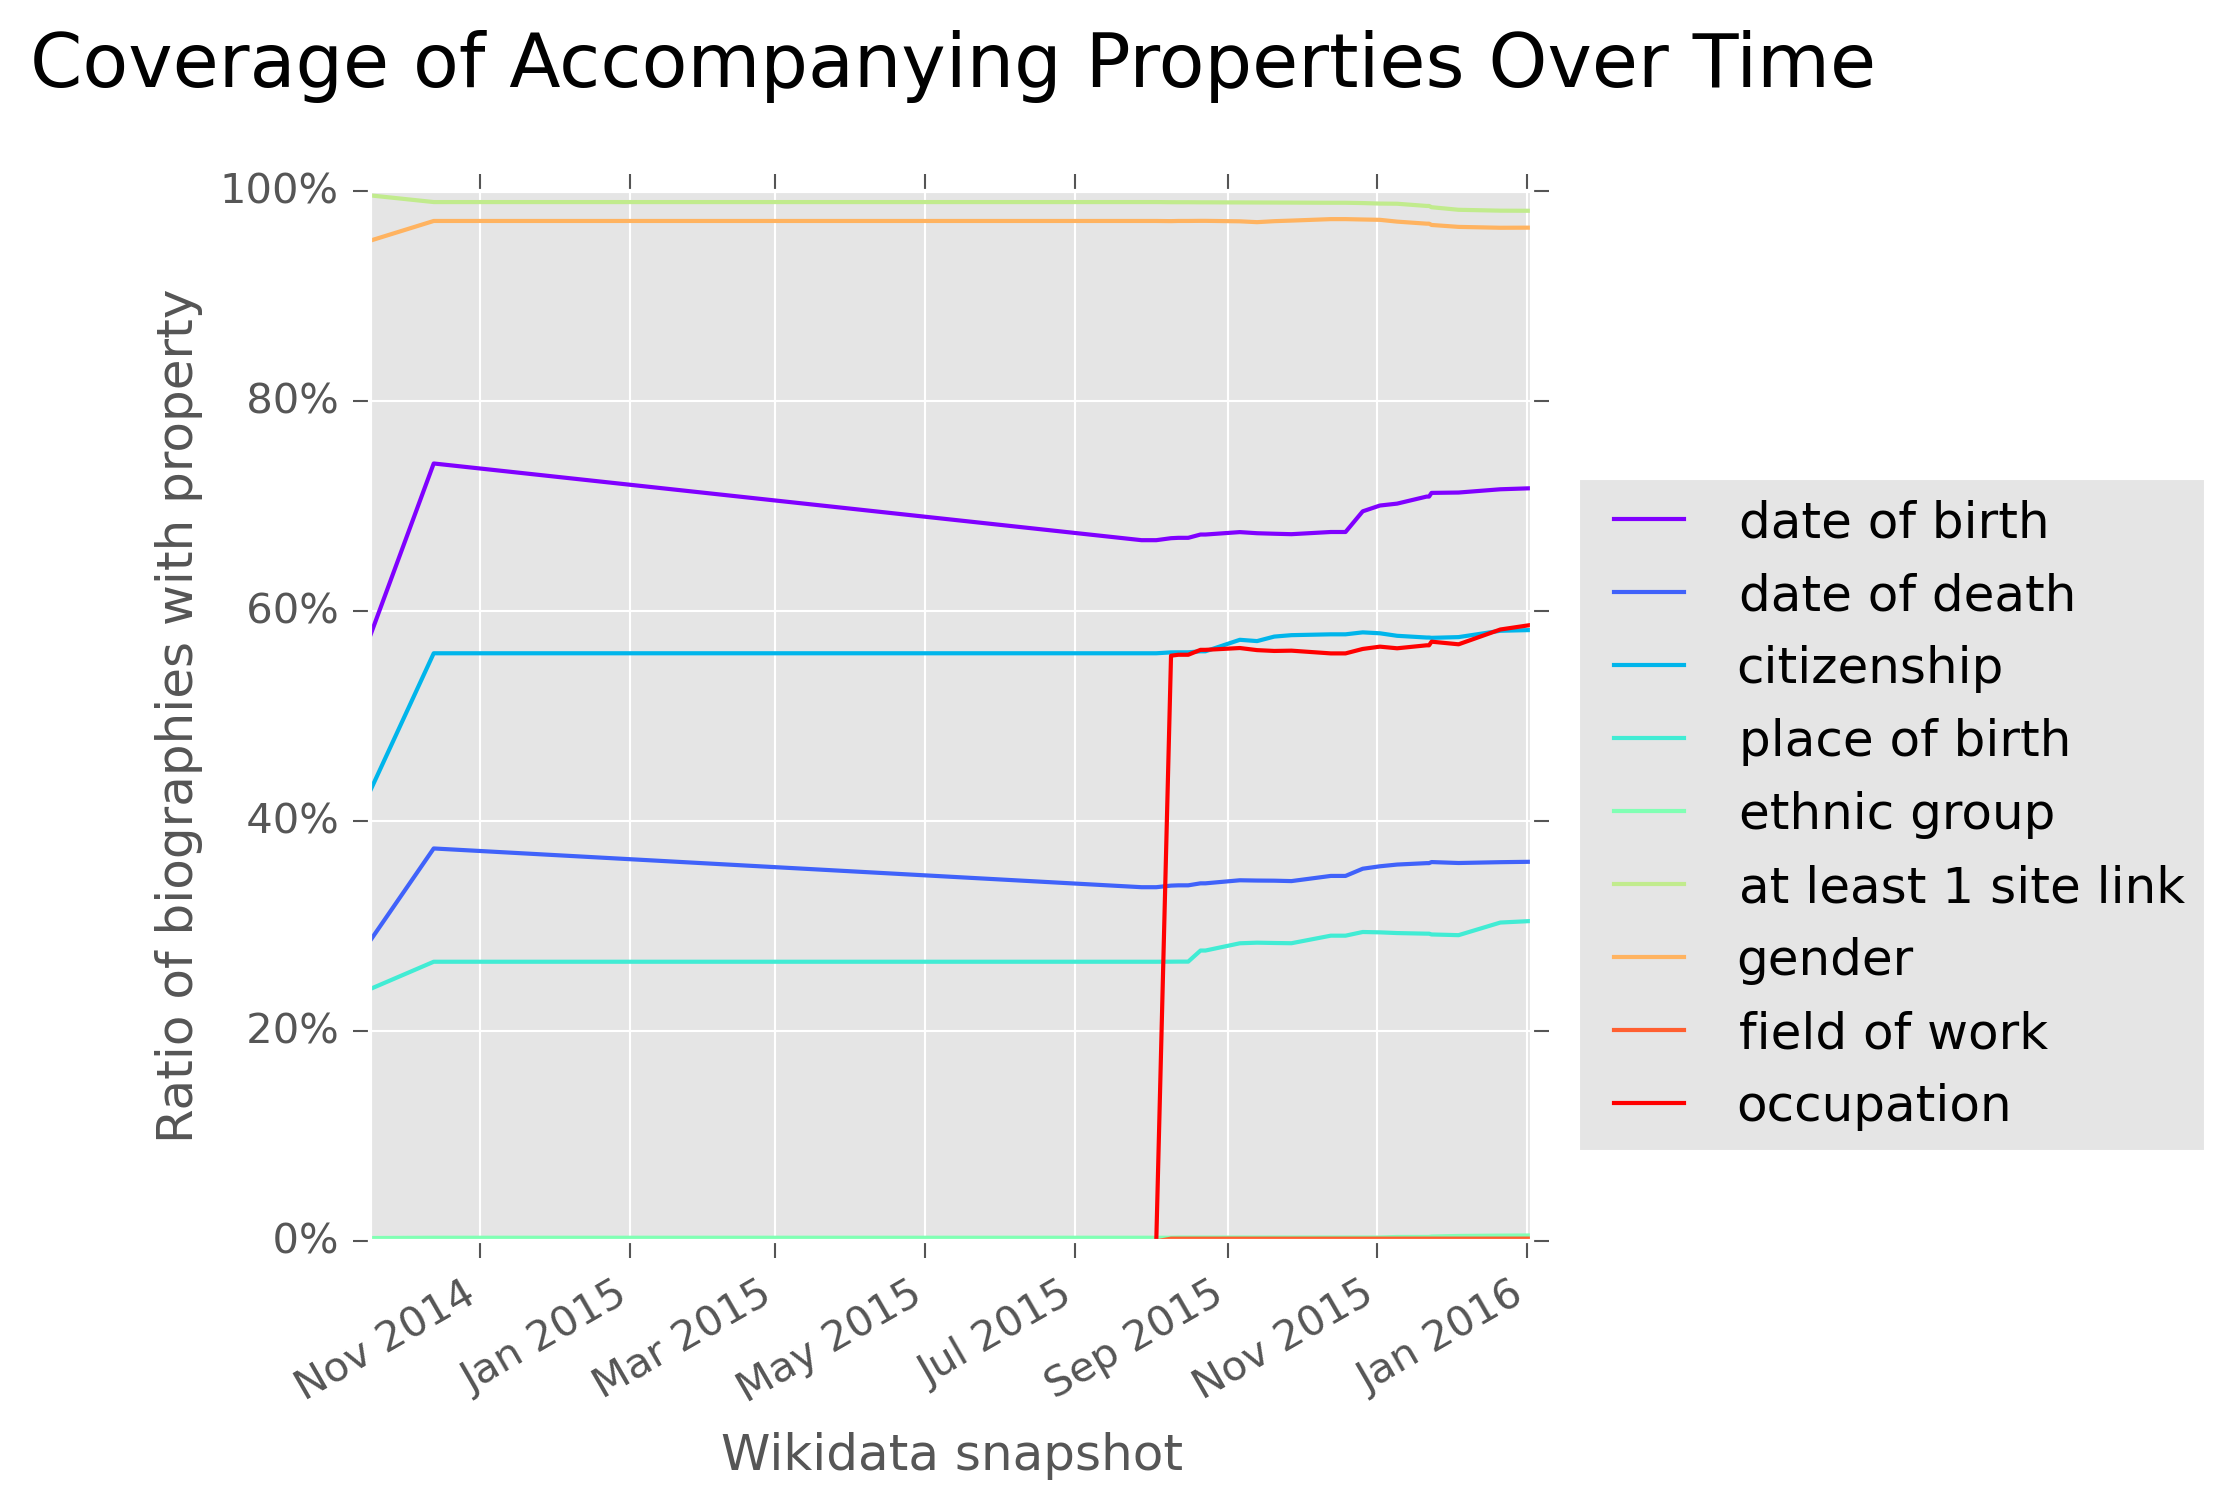
\includegraphics[scale=0.45]{figures/additionalprops.png} 
\caption{Trends of property coverage by Wikidata snapshot. Most humans have at least one Wikipedia article (``site link'') and a recorded gender, other properties are slowly increasing in coverage.}
\label{fig:accompanying}
\end{figure}


\begin{table}
\caption{Change in rates of property coverage for humans}
\begin{tabular}{lrr}
\toprule
{} &  2014-09-17 &  2016-01-03 \\
\midrule
gender               &       95.3\% &       96.5\% \\
date of birth        &       57.6\% &       71.7\% \\
date of death        &       28.6\% &       36.1\% \\
citizenship          &       42.8\% &       58.2\% \\
place of birth       &       24.0\% &       30.5\% \\
ethnic group         &        0.3\% &        0.6\% \\
field of work        &        n/a &        0.3\% \\
occupation           &        n/a &       58.7\% \\
at least 1 site link &       99.6\% &       98.1\% \\
\bottomrule
\end{tabular}
\label{table:accompanying}
\end{table}

\subsection{Data Quality}
Of course the female ratio of biographies is not the only way to characterize the effect of content-focused editing, we might also inquire to the wider quality of biographies in Wikidata. One way to investigate data quality is the coverage of demographic  properties on these biographies. Figure \ref{fig:accompanying} and Table \ref{table:accompanying} show the trend in coverage of all properties at the earliest and latest snapshots. The statistics show that data quality has been increasing across all properties over time. The number of humans with \textit{gender} data increased just 1\% point but is close to complete coverage. In the time domain \textit{date of birth} and \textit{date of death} coverage increased by 14\% points and 7\% points repspectively. Likewise \textit{citizenship} data increased the most, by 15\% points. \textit{place of birth} increased by 6\% points, and \textit{ethnic group} doubled to 0.6\%. \textit{Field of work}, and \textit{occupation} data was not included in our dataset until later, so their growth, while increasing is not precisely comparable.


Curiously the rate of humans having at least on Wikipedia article decreased slightly, but this has an important interpretation. A Wikidata human without a Wikipedia article is known as a ``structural item'', for instance a member of royalty without a Wikipedia article but is needed to make a family tree complete. With the view that a structural item is an artefact from editors paying attention to Wikidata's structure, the decrease in sitelinked humans can also be seen as an increase in data quality. 

There may also be biography articles in Wikipedias that are not recorded as humans in Wikidata, however it is not directly computable how much growth in Wikidata stems from Wikipedia's growth (e.g. a new biography is added), or migration of information to Wikidata (e.g. an existing biography in Wikipedia is marked as a human in Wikidata).


\section{Validation}
Another of our main purposes in creating WHGI was to contribute to the landscape of gender-disparity indicators. In order to gain an idea about how well WHGI reflects the real world we validated our data by comparing it against 3 exogenous datasets. We correlated the WHGI by date of birth versus historical world population trends; WHGI by country versus exogenous gender-disparity indices; and WHGI by occupation versus United States Bureau of Labor Statistics occupation by gender.

\subsection{World Population} Our first validation is a ``sanity check'' to compare the world's population by year to the number of humans in WHGI by year of birth. We conduct this validation even though, the number of people alive and the number of Wikipedia-notable people born are different measures. However if we operate under the assumptions that (a) the proportion of the world population which is Wikipedia-notable is constant over time and (b) that the birth rate is a fixed proportion of the population, then theoretically their curves should share approximately the same shape.

We performed a standard Pearson correlation between the number of people in Wikidata born in a particular year, and the estimated historical world population by the US Census
Bureau\footnote{\url{https://commons.Wikipedia.org/wiki/File:Population_curve.svg}}.
We conducted this correlation for our earliest and latest snapshots - the population statistics of Wikidata at September 2014, and again separately at January 2016. The results in Table \ref{table:worldpop} show a high and significant correlation between real world estimates and Wikidata, at about 0.85. We do see a very minor decrease in correlation over snapshots of 0.007. Overall though the population of Wikidata over time seems very aligned with the World's population over time, so Wikidata at least is a ``sane'' representation of the world.

\begin{table}
\caption{Correlation of number of WHGI by date of birth and world population. Significances are $ ^{**}p\leq 0.01$.}
\label{table:worldpop}
\begin{tabular}{lrrrr}
\toprule
snapshot &  Pearson correlation \\
\midrule
2014-09-17 & 0.852**  \\
2016-01-03 & 0.845**  \\
\bottomrule
\end{tabular}
\end{table}

\subsection{Exogenous Gender-Disparities Indices}
\begin{table}
\caption{WHGI-country correlation to external indices. Correlation is the Spearman $\rho$, and significances are $ ^*p\leq 0.05 $, $ ^{**}p\leq 0.01$.}
\label{table:scores}
\begin{tabular}{lrrrr}
\toprule
snapshot &  GEI &  SIGI &  GGGI &  GDI  \\
\midrule
2014-09-17 &  0.417** &       0.338** &          0.310* &         0.278**  \\
2016-01-03 &  0.457** &       0.402** &          0.386** &         0.299**  \\
\bottomrule
\end{tabular}
\end{table}

WHGI is inspired, in part, by the rich landscape of gender disparity indices. This type of index ranks countries by a measure of gender equality. If we aggregate WHGI by place of birth and citizenship, and look at the female ratio of humans, we too have a sort of country-by-gender equality measure\footnote{Despite having the same by-country unit of analysis with this aggregation WHGI is not an ``index'' like those we compare it to, since an index weights and combines many indicators \cite{rossi_handbook_1980}. }.  We correlated the country rankings of this WHGI aggregation with 4 popular exogenous indices to see how well Wikidata reflects real world gender disparities.

The 4 exogenous indices we used were: The traditional United Nations' Gender Development Index (\textbf{GDI})  \footnote{\url{http://hdr.undp.org/en/content/gender-development-index-gdi}} which considers disparity in income, education, and life expectancy. Social Watch's Gender Equity Index (\textbf{GEI}) \footnote{\url{http://www.socialwatch.org/node/14366}} tries to broaden the scope of the variables by incorportaing education and economic participation, but also stretching into economic and political ``empowerment''. The Global Gender Gap Index (\textbf{GGGI}) \footnote{\url{http://reports.weforum.org/global-gender-gap-report-2014/}} grows yet wider by covering all previous topics and along more detailed dimensions. And most recently  the Social Institutions and Gender Index (\textbf{SIGI}) \footnote{\url{http://www.genderindex.org/ranking}} has attempted to capture disparity in norms, values and attitudes.

Additionally we conducted a calibration step, to find the date of birth threshold which maximized our correlations. In each case the maximizing threshold was found to be between 1900 and 1910. We interpreted the found thresholds as a good sign firstly because the exogenous indices are measures of recent history too, and secondly because it shows a robustness in the way that WHGI relates to exogenous indices.

We repeated the index correlations twice, once using the data  September 2014 snapshot of Wikidata, and then using January 2016 data. That is, we have correlations between rankings of countries given by exogenous indices and Wikidata - at two separate times.

Table \ref{table:scores} shows the correlations with each index, all of which were significant and ranged from 0.278 to 0.457. Affirmingly, when looking at this information through a longitudinal lens, the correlation with every index is increasing over time at which we sampled Wikidata. On the low end the GDI correlation grew by 7.6\%, and on the upper end, the SIGI correlation jumped 24.5\% in the about-a-year time frame between Wikidata snapshots. Because we are using the  female ratio of biographies by country and not the absoulte number these correlation are not growing simply because of increased number of data points.


Previous analyses showed that WHGI being most closely related to GEI, and least to GDI has implications for Wikipedia's notability policy. Where they both measure gender gap in school enrollment, years of schooling, and earned income, GEI additionally measures positions of power, and GDI life expectancy. That means that notablity in Wikipedia is more related to power in society than it is to health status \cite{klein_wikipedia_2015}. This analysis is remains true in 2016, as the order of the strengths of the index correlation has remain unchanged. Still the the strengths of those correlations has increased across all indices, which means that the gender disparities found in WHGI by country are increasingly looking more like these real world gender disparities.


\subsection{Occupation Gender}
The notion of what a human's job or occupation is, we saw in Table \ref{table:accompanying}, well recorded in Wikidata. To answer the question of how representative of the real world Wikidata's gender by occupation is, we compared it to data from the United States Bureau of Labor Statistics (BLS) \footnote{\url{http://www.bls.gov/cps/aa2012/cpsaat11.htm}}. We borrow this ground truth technique from \cite{kay_unequal_2015} who used it to evaluate the gender representation of Google image search results.

Approximately 60\% of our sample have occupation data, and together over 4,000 occupations are represented. The BLS has 332 occupation categories which are at a higher level ontologically than  recorded in Wikidata. Whereas Wikidata might record that someone is a pastry chef, the BLS only has a category for cooks. In order to match the datasets we used Wikidata's internal ontology hierarchy, to generalize the occupation terms. A \textit{subclass of} property exists in Wikidata, that relates items to their more general concept - which we can use for occupations. Wikidata describes that pastry chef is a \textit{subclass of} chef, and that chef is a \textit{sublcass} of cook. 

Our method was to raise the generality of Wikidata occupations until there were less than 500 occupations to ease the matching task. Two authors then matched occupations manually for accuracy and confirmation. We resolved disagreements until the sets were matched. However not all occupations could be matched due to the specificity of the BLS, rendering coverage of Wikidata occupations 57\% complete. The largest occupations in Wikidata were sportsperson and politician, and neither of them had matches in the BLS. In the reverse, there were many BLS occupations for which Wikidata did not have any matching occupations, such as ``lodgings manager''. This outlines a limitation of this validation, that being a lodgings manager does not inherently make you notable for inclusion in Wikipedia. It must be acknowledged too that the BLS data describes the United States whereas WHGI has a worldwide scope, which may explain why we found no significant correlation in the \textit{size} of the matching occupations between the two sets.

Finally we correlated the rankings of the list of most gendered occupations according to WHGI to that of the BLS. We did this for early and late snapshots, but because occupation was not a property that we initially recorded, our first snapshot which included occupation was August 9\textsuperscript{th} 2015.  Table \ref{table:bls} shows the spearman rank correlation found was a significant 0.410, and since then the correlation has increased to 0.473. These are moderate correlations which we claim support a link that Wikidata reflects the real world.

\begin{table}
\caption{Rank correlation of gender ratios by occupation between WHGI and US
Bureau of Labor Statistics. Signficances are $ ^{**}p\leq 0.01$.}
\begin{tabular}{lrrrr}
\toprule
snapshot &  Spearman Rank Correlation \\
\midrule
2015-08-09 & 0.410**  \\
2016-01-03 & 0.473**  \\
\bottomrule
\end{tabular}
\label{table:bls}
\end{table}

\section{Representative Limitations}
The WHGI is measuring two phenomena that we do not disentangle: human development and Wikipedia content development. On the one hand the validation of the dataset tells us how well our measurements capture the various dimensions of gender equality and human development. On the other hand, we are also inspecting how Wikipedia's biography articles and notability policy are based in the real world bias.

To some degree WHGI represents the real world. In each of our validation measures we found high or moderate correlations. Certainly WHGI is not random or isolated, but captures real world dynamics with some distortion. We notice both that WHGI validations are rising over time, and that data quality is rising over time. This can be taken to mean that as Wikidata becomes more complete it is modelling the real world more. There is some justification in using WHGI as a proxy for real-world phenomena, but that proxy is limited by the worldview of Wikipedia editors, and constrained by its notability policies. 

Wikipedia's notability policies require humans to be in positions of power which are systemically biased against women (AUTHOR BLINDED), how then can the rise in women's biographical representation be explained? There could be several possible reasons. At least three factors that affect encyclopedic inclusion are: (1) the rate at which women receive positions of power in the real world, (2) the level of gender bias in Wikipedias' notability policies, and (3) the level of efforts to write about women in Wikipedia. From Figure \ref{fig:changefrb} it seems that there may be some language specific effects.

\section{Impact of WHGI}
There are many Wikipedian communities who's goal it is is to increase the coverage of Women's biographies, for instance: WikiProject Women Scientists \footnote{\url{https://en.wikipedia.org/wiki/Wikipedia:WikiProject_Women_scientists}}, Art + Feminism\footnote{\url{http://art.plusfeminism.org/about/}}, and Women in Red, just to name a few. One concern of these organizations is if their editing efforts are making large scale impacts on the Wikipedia. Luckily Women in Red have been keeping data on their activity levels.

We compared the number of articles added to English Wikipedia by the Women in Red project to the number of biographies added to English Wikipedia marked as women in Wikidata. The correlation between these two activities was 0.657. This medium-high correlation shows that indeed the editing levels of this group are related to the growth of female biographies in Wikidata. This provides a basis to use changes in WHGI as an effectiveness metrics for editing. We hope to find more activity data on the content-focused editing communities, particularly non-English ones to be able to perform ``propensity score matching'' between languages. That is, for a language which has much women-focused editing we could compare the way that language's gender compostion changes against a language which was on a similar trajectory before the change, but had less women-focused editing.

Also for the indirect effects of policy changes and other initiatives that are not specifically article-creation focused we could still measure their change on biography gender. As an example, the gendered implications of changes to a notability policy could be tested using WHGI using the same propensity score matching above. We hope now that this high-level metric is being tracked it will provide an incentive to track more specific editing activity.

Furthermore, applications could be built to detect spikes in creation and deletion of specific demographics of humans. Such a tool could also alert to the presence of unplanned activity, good or bad, which affects the macro-level gender of Wikipedia and Wikidata. Take Figure \ref{fig:genderbylang}, it shows a week where contributions to Nepali Wikipedia are nearly 100\% about women. Likewise, if a week were to show a net-subtraction of female biographies  a community alert could be generated. 

Divorced from Wikipedia entirely, a historian could use the data to determine the gender-disparity levels of a specific place and time. Typically to quantify the gender climate one would rely on the indices like those mentioned in the exogenous indices section. However these indices, are limited to discussing recent history. Our validation showed that our data is in touch with the real world. With this dataset we can quantify a type of gender-disparity of medieval France, ancient Greece, or Ming dynasty China. WHGI is useful in all the same ways that exogenous indices are used, only with a larger timespan. That is certainly a novel approach not possible before Wikidata.

Yet another new avenue this dataset opens is in the gender-disparity of a language. A linguist could use WHGI aggregated by language to quantify the gendered-ness of a language. Furthermore with the date of birth and death information, the linguist could see how languages have focused on gender differently over time. Potentially this could lend evidence to another theory of language that comes from their native methods. 

WHGI is, in essence, a biographic database. The data can not only provide insights on gender-related disparity, but also other disparities such as culture disparities, citizen disparities and ethnic group disparities, etc.  

\section{Conclusion and Future Work}
We made the Wikidata Human Gender Indicators (WHGI), a biographic database for researchers wishing to incorporate gender data along dimensions of time, space and occupation. Based off of Wikidata and Wikipedia it can most obviously be used by those communities to monitor the effects of focused editing and biases in their content. We also validated the indicators with measures of the real world, such as population, country-based gender disparities, and occupations. These validations showed that the WHGI is significantly correlated to real world demographics and gender disparities. We also showed that data quality of Wikidata has been increasing. Data quality and correlations increasing together is particularly encouraging as support for using WHGI as a tool. WHGI is freely available for download, we have outlined some of the potential ways in which it could be used, and hope that many more are thought of by others.

We hope to continue running the open source project in service of the Wikipedia and research communities seeking to statistically describe gender disparities. The ways in which we expand WHGI we hope will be directed by user's feedback.

\section{ Acknowledgments}
We are especially grateful to the Wikimedia Foundation for funding us through an Individual Engagement Grant. [GRANT BLINDED].

We are also especially grateful to the Wikidata and Wikidata Toolkit teams.

Finally we acknowledge the hard work done by Wikimedians in  countering systemic bias.


%
% The following two commands are all you need in the
% initial runs of your .tex file to
% produce the bibliography for the citations in your paper.
\bibliographystyle{abbrv}
\bibliography{wigi-dataset-opensym}  % sigproc.bib 
\end{document}
